%!TeX encoding = UTF-8
%!TeX program = xelatex
\documentclass[notheorems, aspectratio=54]{beamer}
% aspectratio: 1610, 149, 54, 43(default), 32

\usepackage{latexsym}
\usepackage{amsmath,amssymb}
\usepackage{mathtools}
\usepackage{color,xcolor}
\usepackage{graphicx}

% \usepackage{algorithm}
\usepackage[ruled]{algorithm2e}
\SetKw{KwInit}{Init:}
\SetKw{KwReturn}{Return}

\usepackage{amsthm}
\usepackage{lmodern} % 解决 font warning
% \usepackage[UTF8]{ctex}
\usepackage{animate} % insert gif

\usepackage{lipsum} % To generate test text 
\usepackage{ulem} % 下划线,波浪线

\usepackage{listings} % display code on slides; don't forget [fragile] option after \begin{frame}

\usepackage{booktabs}
\usepackage{multirow}
\usepackage{bbding}

% ----------------------------------------------
% tikx
\usepackage{framed}
\usepackage{tikz}
\usepackage{pgf}
\usetikzlibrary{calc,trees,positioning,arrows,chains,shapes.geometric,%
    decorations.pathreplacing,decorations.pathmorphing,shapes,%
    matrix,shapes.symbols}
\pgfmathsetseed{1} % To have predictable results
% Define a background layer, in which the parchment shape is drawn
\pgfdeclarelayer{background}
\pgfsetlayers{background,main}

% define styles for the normal border and the torn border
\tikzset{
  normal border/.style={orange!30!black!10, decorate, 
     decoration={random steps, segment length=2.5cm, amplitude=.7mm}},
  torn border/.style={orange!30!black!5, decorate, 
     decoration={random steps, segment length=.5cm, amplitude=1.7mm}}}

% Macro to draw the shape behind the text, when it fits completly in the
% page
\def\parchmentframe#1{
\tikz{
  \node[inner sep=2em] (A) {#1};  % Draw the text of the node
  \begin{pgfonlayer}{background}  % Draw the shape behind
  \fill[normal border] 
        (A.south east) -- (A.south west) -- 
        (A.north west) -- (A.north east) -- cycle;
  \end{pgfonlayer}}}

% Macro to draw the shape, when the text will continue in next page
\def\parchmentframetop#1{
\tikz{
  \node[inner sep=2em] (A) {#1};    % Draw the text of the node
  \begin{pgfonlayer}{background}    
  \fill[normal border]              % Draw the ``complete shape'' behind
        (A.south east) -- (A.south west) -- 
        (A.north west) -- (A.north east) -- cycle;
  \fill[torn border]                % Add the torn lower border
        ($(A.south east)-(0,.2)$) -- ($(A.south west)-(0,.2)$) -- 
        ($(A.south west)+(0,.2)$) -- ($(A.south east)+(0,.2)$) -- cycle;
  \end{pgfonlayer}}}

% Macro to draw the shape, when the text continues from previous page
\def\parchmentframebottom#1{
\tikz{
  \node[inner sep=2em] (A) {#1};   % Draw the text of the node
  \begin{pgfonlayer}{background}   
  \fill[normal border]             % Draw the ``complete shape'' behind
        (A.south east) -- (A.south west) -- 
        (A.north west) -- (A.north east) -- cycle;
  \fill[torn border]               % Add the torn upper border
        ($(A.north east)-(0,.2)$) -- ($(A.north west)-(0,.2)$) -- 
        ($(A.north west)+(0,.2)$) -- ($(A.north east)+(0,.2)$) -- cycle;
  \end{pgfonlayer}}}

% Macro to draw the shape, when both the text continues from previous page
% and it will continue in next page
\def\parchmentframemiddle#1{
\tikz{
  \node[inner sep=2em] (A) {#1};   % Draw the text of the node
  \begin{pgfonlayer}{background}   
  \fill[normal border]             % Draw the ``complete shape'' behind
        (A.south east) -- (A.south west) -- 
        (A.north west) -- (A.north east) -- cycle;
  \fill[torn border]               % Add the torn lower border
        ($(A.south east)-(0,.2)$) -- ($(A.south west)-(0,.2)$) -- 
        ($(A.south west)+(0,.2)$) -- ($(A.south east)+(0,.2)$) -- cycle;
  \fill[torn border]               % Add the torn upper border
        ($(A.north east)-(0,.2)$) -- ($(A.north west)-(0,.2)$) -- 
        ($(A.north west)+(0,.2)$) -- ($(A.north east)+(0,.2)$) -- cycle;
  \end{pgfonlayer}}}

% Define the environment which puts the frame
% In this case, the environment also accepts an argument with an optional
% title (which defaults to ``Example'', which is typeset in a box overlaid
% on the top border
\newenvironment{parchment}[1][Example]{%
  \def\FrameCommand{\parchmentframe}%
  \def\FirstFrameCommand{\parchmentframetop}%
  \def\LastFrameCommand{\parchmentframebottom}%
  \def\MidFrameCommand{\parchmentframemiddle}%
  \vskip\baselineskip
  \MakeFramed {\FrameRestore}
  \noindent\tikz\node[inner sep=1ex, draw=black!20,fill=white, 
          anchor=west, overlay] at (0em, 2em) {\sffamily#1};\par}%
{\endMakeFramed}

% ----------------------------------------------

\mode<presentation>{
    \usetheme{CambridgeUS}
    % Boadilla CambridgeUS
    % default Antibes Berlin Copenhagen
    % Madrid Montpelier Ilmenau Malmoe
    % Berkeley Singapore Warsaw
    \usecolortheme{beaver}
    % beetle, beaver, orchid, whale, dolphin
    \useoutertheme{infolines}
    % infolines miniframes shadow sidebar smoothbars smoothtree split tree
    \useinnertheme{circles}
    % circles, rectanges, rounded, inmargin
}
% 设置 block 颜色
% \setbeamercolor{block title}{bg=red!30,fg=white}
\setbeamercolor{block title}{bg=gray!10,fg=darkred}

\newcommand{\reditem}[1]{\setbeamercolor{item}{fg=red}\item #1}

% 缩放公式大小
\newcommand*{\Scale}[2][4]{\scalebox{#1}{\ensuremath{#2}}}

% 解决 font warning
\renewcommand\textbullet{\ensuremath{\bullet}}

% number the figures and tables
\setbeamertemplate{caption}[numbered]

% bibliography
% \setbeamertemplate{bibliography item}[text]
\usepackage[backend=bibtex,style=numeric,sorting=none]{biblatex}
\addbibresource{mybib} %BibTeX数据文件及位置
\setbeamerfont{footnote}{size=\tiny}


% ---------------------------------------------------------------------
% flow chart
% \tikzset{
%     >=stealth',
%     punktchain/.style={
%         rectangle, 
%         rounded corners, 
%         % fill=black!10,
%         draw=white, very thick,
%         text width=6em,
%         minimum height=2em, 
%         text centered, 
%         on chain
%     },
%     largepunktchain/.style={
%         rectangle,
%         rounded corners,
%         draw=white, very thick,
%         text width=10em,
%         minimum height=2em,
%         on chain
%     },
%     line/.style={draw, thick, <-},
%     element/.style={
%         tape,
%         top color=white,
%         bottom color=blue!50!black!60!,
%         minimum width=6em,
%         draw=blue!40!black!90, very thick,
%         text width=6em, 
%         minimum height=2em, 
%         text centered, 
%         on chain
%     },
%     every join/.style={->, thick,shorten >=1pt},
%     decoration={brace},
%     tuborg/.style={decorate},
%     tubnode/.style={midway, right=2pt},
%     font={\fontsize{10pt}{12}\selectfont},
% }
% ---------------------------------------------------------------------

% code setting
\lstset{
    language=C++,
    basicstyle=\ttfamily\footnotesize,
    keywordstyle=\color{red},
    breaklines=true,
    xleftmargin=2em,
    numbers=left,
    numberstyle=\color[RGB]{222,155,81},
    frame=leftline,
    tabsize=4,
    breakatwhitespace=false,
    showspaces=false,               
    showstringspaces=false,
    showtabs=false,
    morekeywords={Str, Num, List},
}

% ---------------------------------------------------------------------

%% preamble
\title[]{General Multi-view Neural Network}
\subtitle{Current Research}
\author{Jiyuan}
\institute[NUDT]{liujiyuan13@nudt.edu.cn}

% -------------------------------------------------------------

\begin{document}

\section{Title}
%% title frame
\begin{frame}
    \titlepage
\end{frame}

%% normal frame
\section{Current Research}

\begin{frame}
    
    \centering
    \LARGE Current research
    
\end{frame}

\subsection{Latent Multi-view Subspace Clustering}

\begin{frame} \frametitle{Latent Multi-view Subspace Clustering \footnote{Zhang et. al. \textcolor{blue}{Latent Multi-view Subspace Clustering}. IEEE CVPR, 2017.}}

Overview:

\begin{figure}
\centering
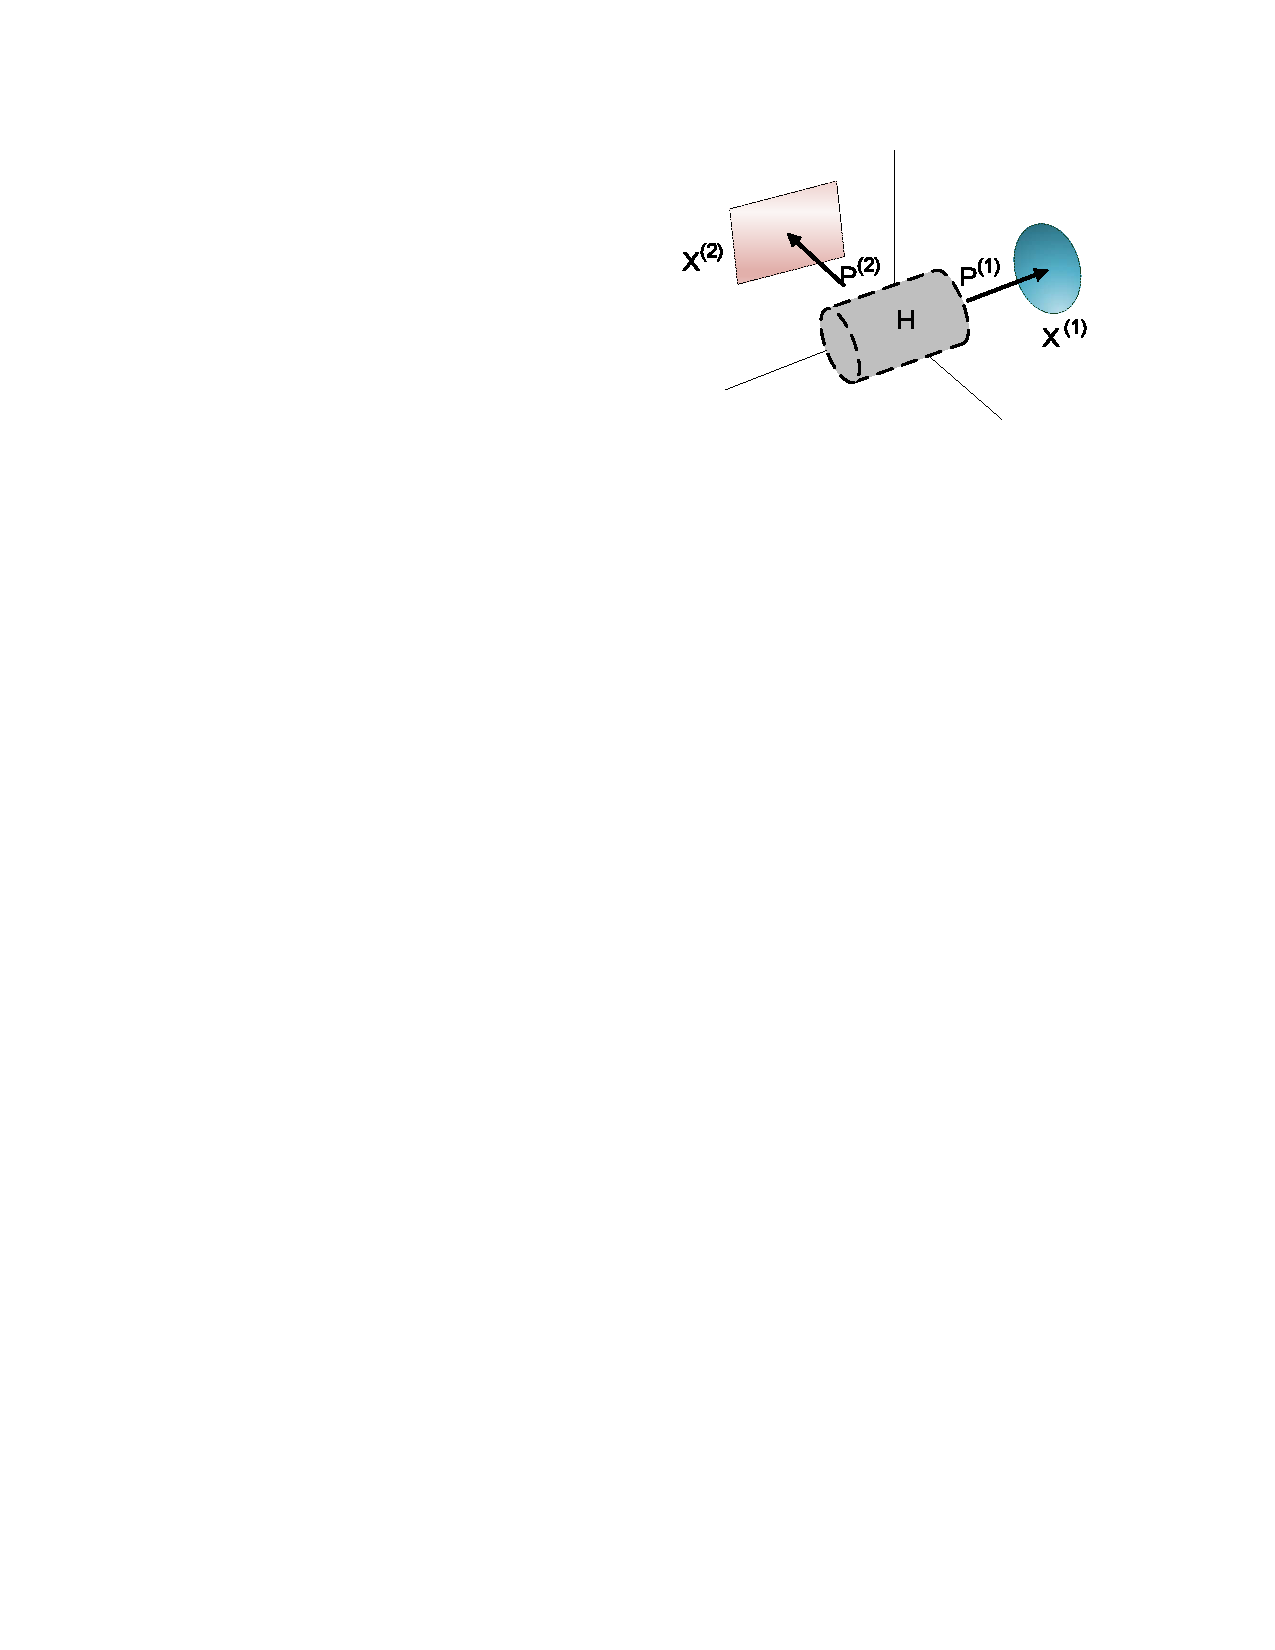
\includegraphics[width=0.6\textwidth]{./fig/overview_lmsc.pdf}
\caption{Overview of LMSC. Observations $\{\mathbf{X}_v\}_{v=1}^V\;(V\geq 2)$ corresponding to different views are partially projected by $\{\mathbf{P}_v\}_{v=1}^V$ from one underlying latent representation H.}
\label{fig:overview_lmsc}
\end{figure}

\end{frame}


\begin{frame} \frametitle{Latent Multi-view Subspace Clustering}

Formulation:

\begin{equation}
\begin{split}
  \min_{\mathbf{P}, \mathbf{H}, \mathbf{Z}, \mathbf{E}_h, \mathbf{E}_r}\; & \|\mathbf{E}\|_{2,1} + \lambda\|\mathbf{Z}\|_* \\
  s.t.\; & \mathbf{X} = \mathbf{P}\mathbf{H} + \mathbf{E}_h,\; \mathbf{H} = \mathbf{H}\mathbf{Z} + \mathbf{E}_r, \\
  & \mathbf{E} = [\mathbf{E}_h;\mathbf{E}_r], \mathbf{P}\mathbf{P}^\top = \mathbf{I}, 
\end{split}
\end{equation}
in which
\begin{equation}
\begin{split}
  \mathbf{X} = \begin{bmatrix} \mathbf{X}_1 \\ \cdots \\ \mathbf{X}_V \end{bmatrix},\; \mathbf{P} = \begin{bmatrix} \mathbf{P}_1 \\ \cdots \\ \mathbf{P}_V \end{bmatrix}. 
\end{split}
\end{equation}

\end{frame}


\subsection{Generalized Latent Multi-view Subspace Clustering}

\begin{frame} \frametitle{Generalized Latent Multi-view Subspace Clustering \footnote{Zhang et. al. \textcolor{blue}{Generalized Latent Multi-view Subspace Clustering}. IEEE TPAMI, 2019.}}

Overview:

\begin{figure}
\centering
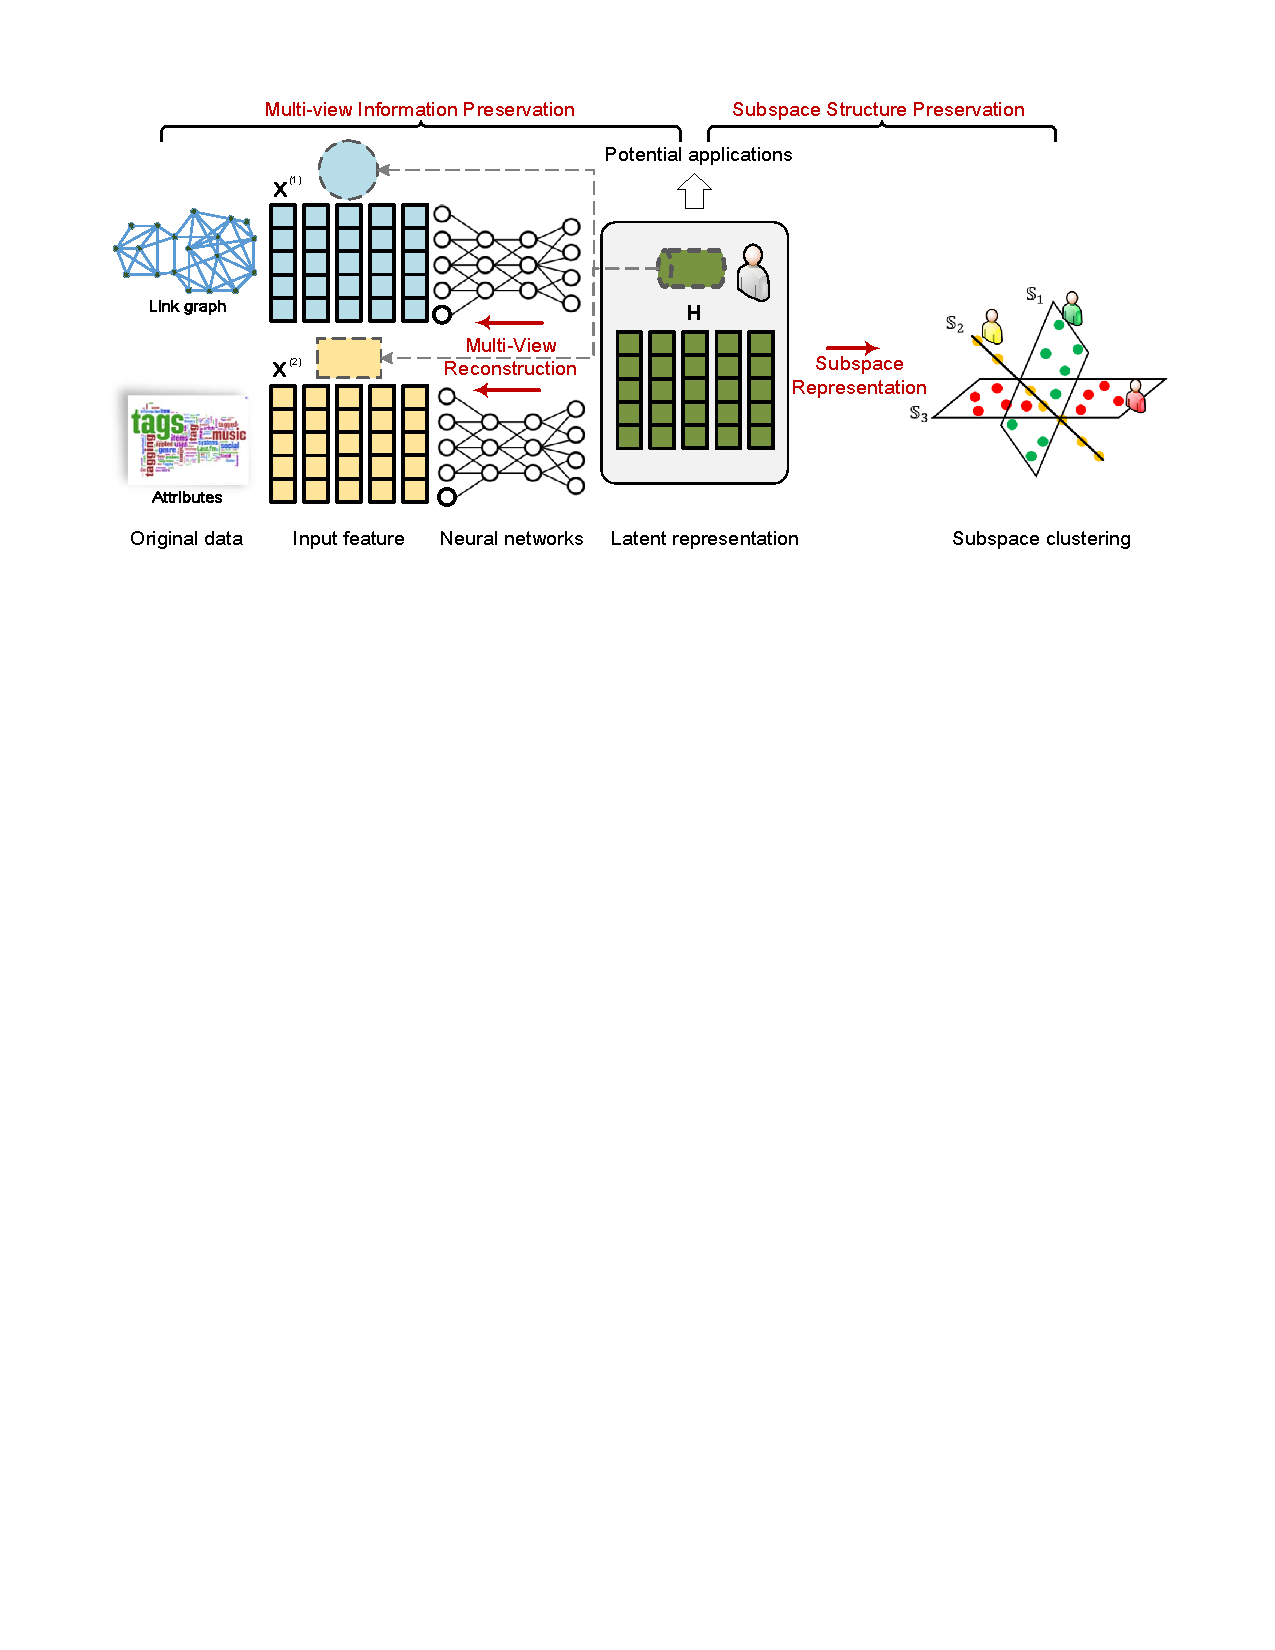
\includegraphics[width=0.95\textwidth]{./fig/overview_glmsc.pdf}
\caption{Overview of gLMSC. The latent representation non-linearly encodes the information from multiple views with neural networks for uncovering the data distribution in subspaces.}
\label{fig:overview_lmsc}
\end{figure}

\end{frame}

\begin{frame} \frametitle{Generalized Latent Multi-view Subspace Clustering}

Formulation:

\begin{equation}
\begin{split}
  \min_{\{\boldsymbol{\theta_v}\}_{v=1}^V, \mathbf{H}, \mathbf{Z}}\; & \ell(\mathbf{H}, \mathbf{H}\mathbf{Z}) + \sum_{v=1}^V\alpha_vd_v(\mathbf{X}_v, g_{\boldsymbol{\theta}_v}(\mathbf{H})) + \lambda \Omega(\mathbf{Z}) \\
  s.t.\; & g_{\boldsymbol{\theta}_v}(\mathbf{H}) = \mathbf{W}_{(k,v)}f(\mathbf{W}_{(k-1,v)} \cdots f(\mathbf{W}_{(1,v)}\mathbf{H})).
\end{split}
\end{equation}

Instance:
\begin{equation}
\begin{split}
  & \ell(\mathbf{H}, \mathbf{H}\mathbf{Z}) = \frac{1}{2} \|\mathbf{H} - \mathbf{H}\mathbf{Z}\|_F^2 \\
  & d_v(\mathbf{X}_v, g_{\boldsymbol{\theta}_v}(\mathbf{H})) = \frac{1}{2} \|\mathbf{X}_v - \mathbf{W}_{(2,v)}f(\mathbf{W}_{(1,v)}\mathbf{H})\|_F^2 \\
  & \Omega(\mathbf{Z}) = \|\mathbf{Z}\|_*.
\end{split}
\end{equation}


\end{frame}


\subsection{CPM-Nets: Cross Partial Multi-View Networks}

\begin{frame} \frametitle{CPM-Nets: Cross Partial Multi-View Networks \footnote{Zhang et. al. \textcolor{blue}{CPM-Nets: Cross Partial Multi-View Networks}. NeurIPS, 2020.}}

Overview:

\begin{figure}
\centering
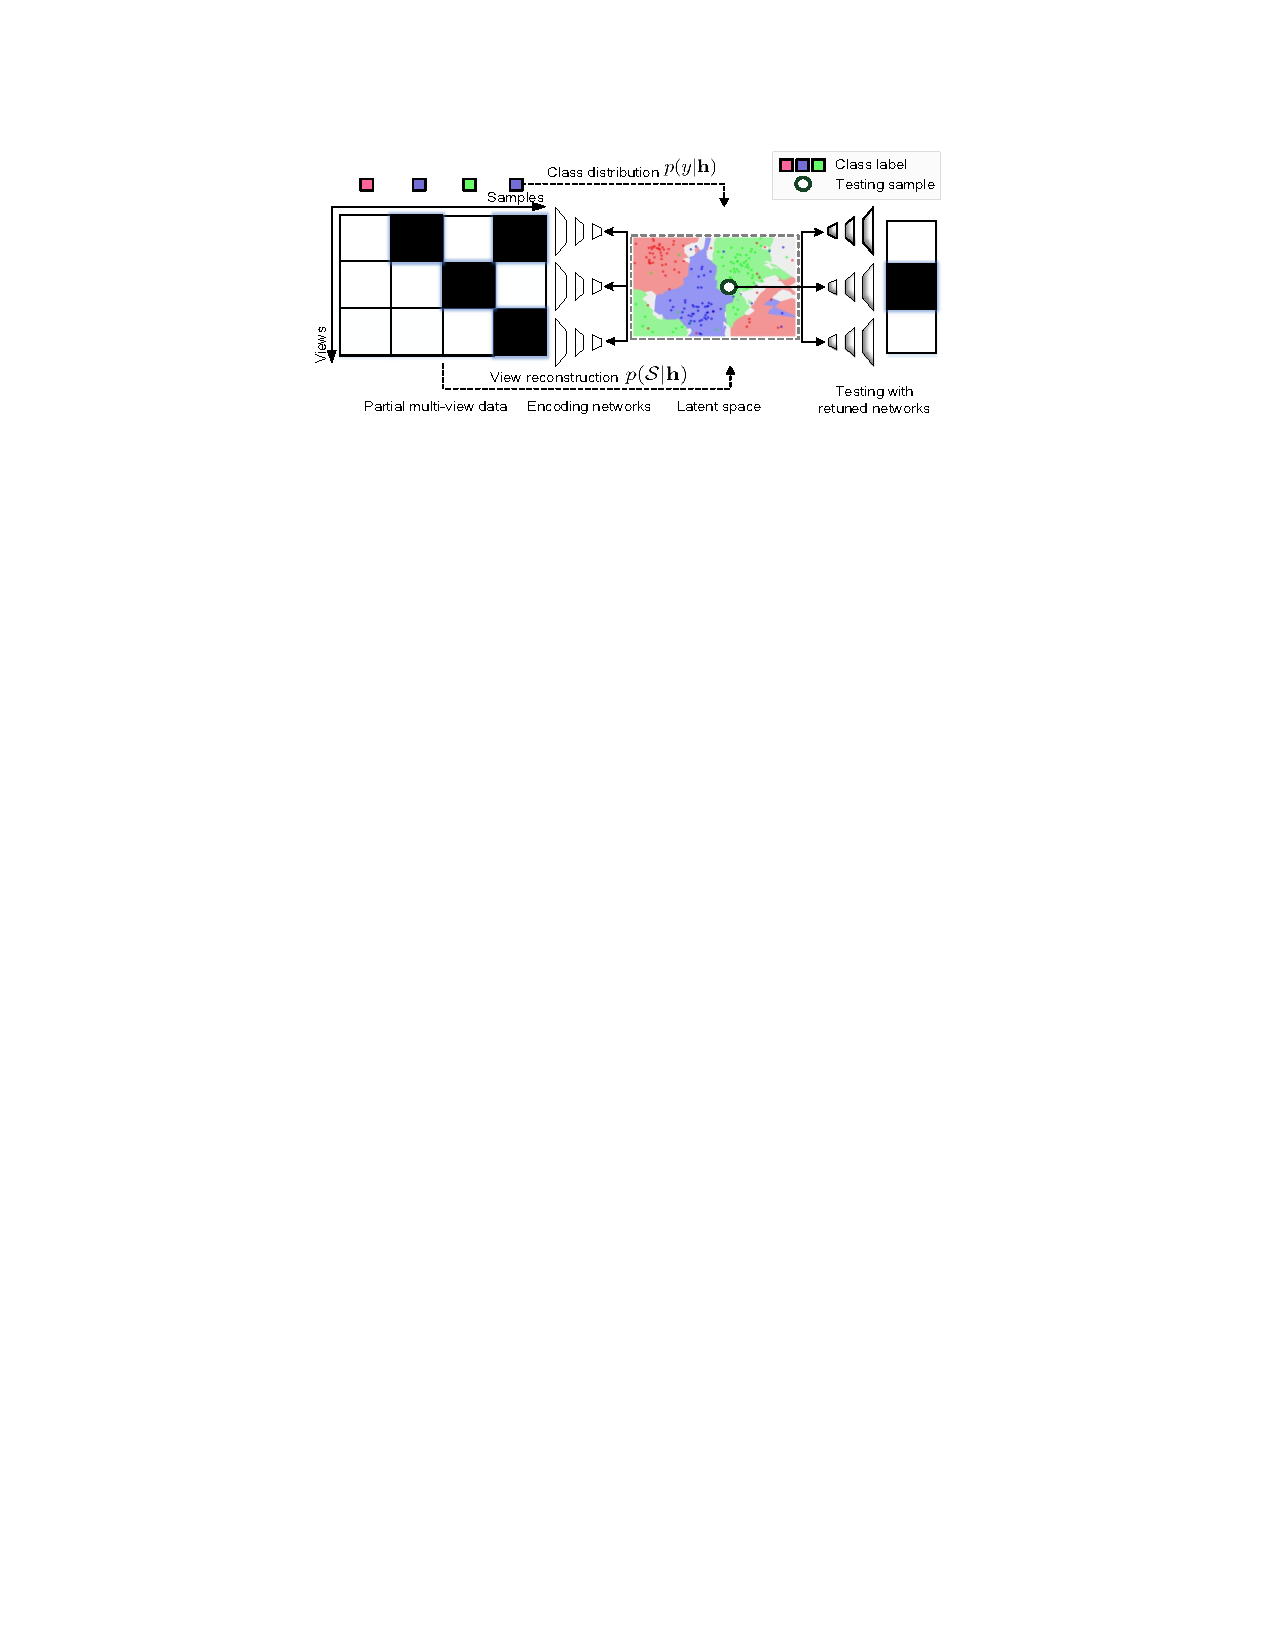
\includegraphics[width=0.95\textwidth]{./fig/overview_cpmnet.pdf}
\caption{Overview of CPMnet.  Given multi-view data with missing views (black blocks), the encoding networks degrade the complete latent representation into the available views (white blocks).}
\label{fig:overview_lmsc}
\end{figure}


\end{frame}


\begin{frame} \frametitle{CPM-Nets: Cross Partial Multi-View Networks}

Formulation:

\begin{equation}
\begin{split}
  \min_{\{\mathbf{h}_n\}_{n=1}^N, \boldsymbol{\Theta}_r}\; \frac{1}{N}\sum_{n=1}^N \ell_r(\mathcal{S}_n, \mathbf{h}_n; \boldsymbol{\Theta}_r) + \lambda \ell_c(y_n, y, \mathbf{h}_n)
\end{split}
\end{equation}

in which 
\begin{equation}
\begin{split}
  & \ell_r(\mathcal{S}_n, \mathbf{h}_n; \boldsymbol{\Theta}_r) = \sum_{v=1}^V s_{nv}\|f_v(\mathbf{h}_n; \boldsymbol{\Theta}_r^{(v)}) - \mathbf{x}_n^{(v)}\|^2 \\
  & \ell_c(y_n, y, \mathbf{h}_n) = \max_{y\in \mathcal{Y}} \left( 0, \Delta (y_n, y) + \mathbb{E}_{\mathbf{h}\sim\mathcal{T}(y)} F(\mathbf{h}, \mathbf{h}_n) - \mathbb{E}_{\mathbf{h}\sim\mathcal{T}(y_n)} F(\mathbf{h}, \mathbf{h}_n) \right) \\
  & \Delta (y_n, y) = \Delta (y_n, g(\mathbf{h}_n;\boldsymbol{\Theta}_c)) \\
  & g(\mathbf{h}_n;\boldsymbol{\Theta}_c) = \arg\max_{y\in\mathcal{Y}} \mathbb{E}_{\mathbf{h}\sim\mathcal{T}(y)} F(\mathbf{h}, \mathbf{h}_n) \\
  & F(\mathbf{h}, \mathbf{h}_n) = \phi (\mathbf{h}; \boldsymbol{\Theta}_c)^\top\phi (\mathbf{h}; \boldsymbol{\Theta}_c)
\end{split}
\end{equation}

\end{frame}


\begin{frame} \frametitle{CPM-Nets: Cross Partial Multi-View Networks}

\begin{algorithm}[H]
\small
  \# Training \\
    \KwIn{Partial multi-view dataset: $\mathcal{D}=\{\mathcal{S}_n,y_n\}_{n=1}^N$, parameter $\lambda$.}
        Initialize $\{\mathbf{h}_n\}_{n=1}^N$ and $\{\boldsymbol{\Theta}_r^{(v)}\}_{v=1}^V$. \\
        \While{not convergence}{
          \For{$v=1:V$}{
            Update the network parameters $\boldsymbol{\Theta}_r^{(v)}$ with $\ell_r(\mathcal{S}_n,\mathbf{h}_n;\boldsymbol{\Theta}_r)$;
          }
          \For{$n=1:N$}{
            Update the representation $\mathbf{h}_n$ with $\ell_r(\mathcal{S}_n,\mathbf{h}_n;\boldsymbol{\Theta}_r) + \lambda \ell_c(y_n,y,\mathbf{h}_n)$;
          }
        }
    \KwOut{network parameters $\{\boldsymbol{\Theta}_r^{(v)}\}_{v=1}^V$ and latent representations $\{\mathbf{h}_n\}_{n=1}^N$}
  \# Testing \\
    Train the retuned networks $(\{\boldsymbol{\Theta}_r^{(v)}\}_{v=1}^V)$ for test;  \\
    Calculate the latent representation for test instance; \\
    Classify the test instance with $y=\arg\max_{y\in\mathcal{Y}}\mathbb{E}_{\mathbf{h}\sim\mathcal{T}(y)}F(\mathbf{h}, \mathbf{h}_{test})$.
\caption{CPM-Nets: Cross Partial Multi-View Networks}
\label{alg:cpm_nets}
\end{algorithm}


\end{frame}


\subsection{Deep Partial Multi-view Learning}

\begin{frame} \frametitle{Deep Partial Multi-view Learning \footnote{Zhang et. al. \textcolor{blue}{Deep Partial Multi-view Learning}. IEEE TPAMI, 2021.}}

Overview:

\begin{figure}
\centering
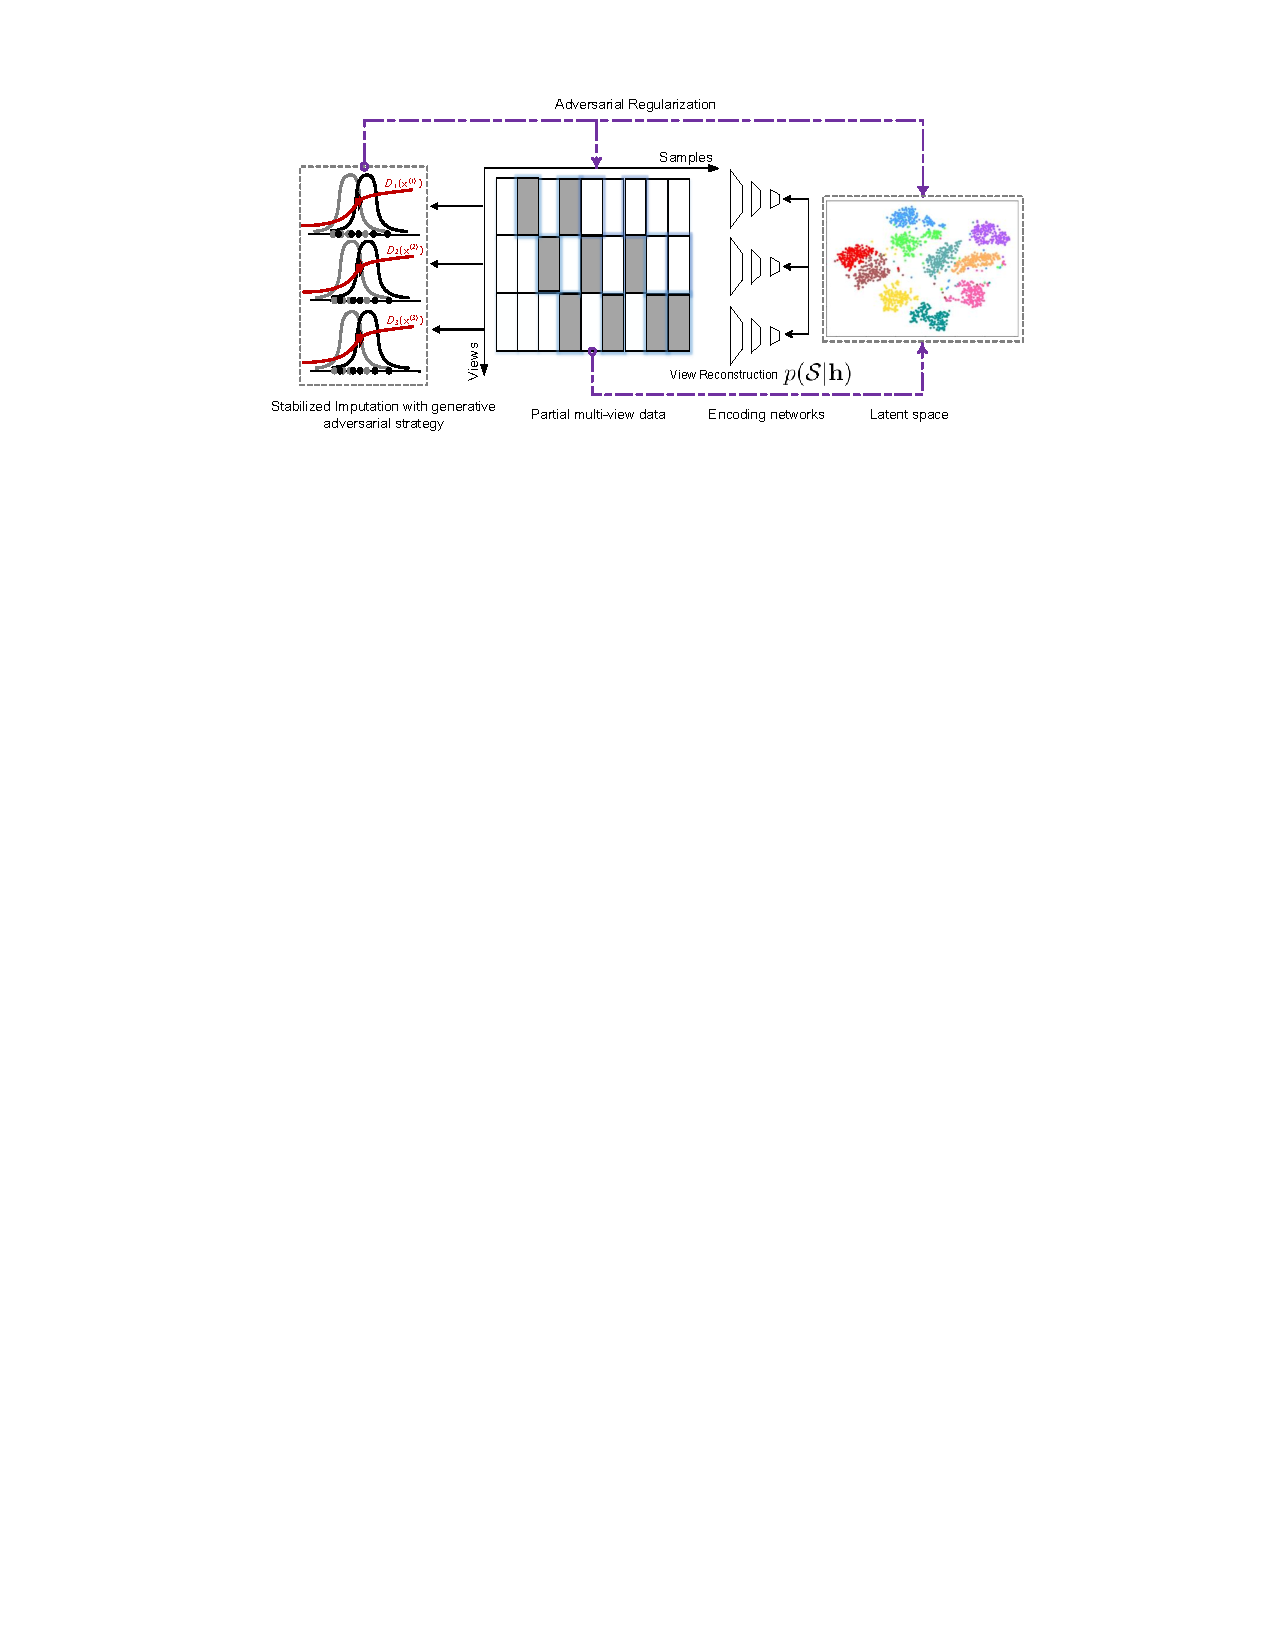
\includegraphics[width=0.95\textwidth]{./fig/overview_cpm_gan.pdf}
\caption{Overview of CPM-GAN. The latent representation learning and missing data imputation equipped with adversarial strategy are jointly conducted to improve each other.}
\label{fig:overview_cpm_gan}
\end{figure}


\end{frame}


\begin{frame} \frametitle{Deep Partial Multi-view Learning}

% GAN Objective:

% \begin{equation}
% \begin{split}
%   \min_G\max_D V(D, G) = \mathbb{E}_{\mathbf{x}\sim p_{data}(\mathbf{x})}[\log D(\mathbf{x})] + \mathbb{E}_{\mathbf{z}\sim p_{\mathbf{z}}(\mathbf{z})}[\log(1-D(G(\mathbf{z})))]
% \end{split}
% \end{equation}

Formulation:

\begin{equation}
\begin{split}
  \mathcal{L} = \min_G\max_D\min_{\mathbf{h}} (\mathcal{L}_{adv} + \mathcal{L}_r)
\end{split}
\end{equation}

in which 

\begin{equation}
\begin{split}
  \mathcal{L}_{adv} = & \sum_{n=1}^N\sum_{v=1}^V\sum_{i=1}^I(1-s_{nv})[\log D_v(\mathbf{x}_i^{(v)};\boldsymbol{\Theta}_d^{(v)})  \\
  & + \log(1-D_v(G_v(\mathbf{h}_n;\boldsymbol{\Theta}_g^{(v)});\boldsymbol{\Theta}_d^{(v)}))]; \\
  \mathcal{L}_{r} = & \sum_{n=1}^N\sum_{v=1}^Vs_{nv}\|G_v(\mathbf{h}_n;\boldsymbol{\Theta}_g^{(v)}) - \mathbf{x}_n^{(v)} \|^2.
\end{split}
\end{equation}


\end{frame}


\begin{frame} \frametitle{Deep Partial Multi-view Learning}

\begin{algorithm}[H]
\small
    \KwIn{Partial multi-view dataset: $\mathcal{D}=\{\mathcal{S}_n\}_{n=1}^N$.}
        Initialize $\{\mathbf{h}_n\}_{n=1}^N$, $\{\boldsymbol{\Theta}_g^{(v)}\}_{v=1}^V$ and $\{\boldsymbol{\Theta}_d^{(v)}\}_{v=1}^V$. \\
        \While{not convergence}{
          \For{$v=1:V$}{
            Update the discriminator parameters $\boldsymbol{\Theta}_d^{(v)}$ with gradient descent;
          }
          \For{$v=1:V$}{
            Update the generator parameters $\boldsymbol{\Theta}_g^{(v)}$ with gradient descent;
          }
          \For{$n=1:N$}{
            Update the representation $\mathbf{h}_n$ with gradient descent;
          }
        }
    \KwOut{$\{\mathbf{h}_n\}_{n=1}^N$, $\{\boldsymbol{\Theta}_d^{(v)}\}_{v=1}^V$ and $\{\boldsymbol{\Theta}_g^{(v)}\}_{v=1}^V$}
\caption{Deep Partial Multi-view Learning - CPM-GAN}
\label{alg:cpm_gan}
\end{algorithm}


\end{frame}


\subsection{CVOID-19 Detection with Multi-view Learning}

\begin{frame} \frametitle{CVOID-19 Detection with Multi-view Learning \footnote{Kang et. al. \textcolor{blue}{Diagnosis of Coronavirus Disease 2019 (COVID-19) with Structured Latent Multi-View Representation Learning}. IEEE TMI, 2021.}}

Overview:

\begin{figure}
\centering
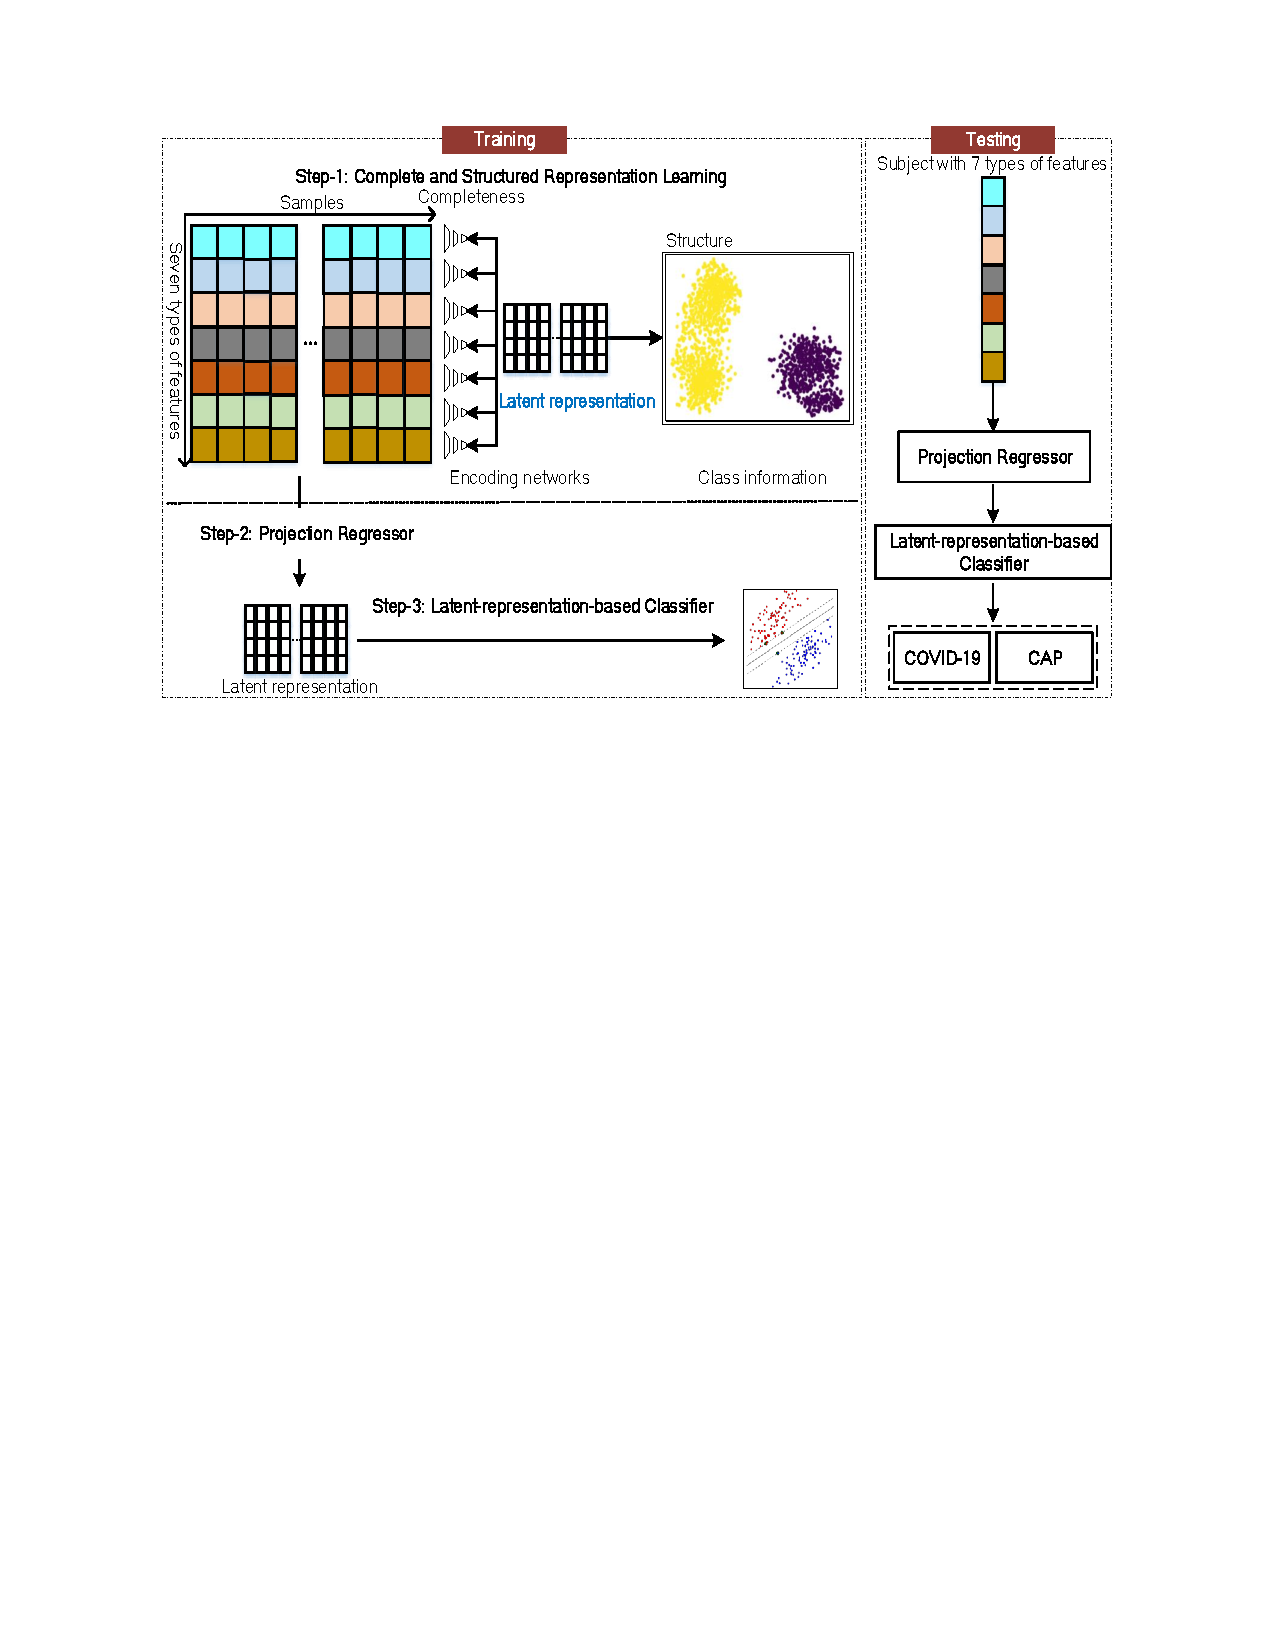
\includegraphics[width=0.8\textwidth]{./fig/overview_covid19.pdf}
\caption{Overview of the latent-representation-based diagnosis framework. }
\label{fig:overview_covid19}
\end{figure}


\end{frame}


\section{Thought}

\begin{frame}
    
    \centering
    \LARGE Thought
    
\end{frame}

\subsection{Advantages and Shortcomings}

\begin{frame} \frametitle{Advantages and Shortcomings}

Advantages:
\begin{enumerate}
  \item Native framework to integrate multi-view information;
  \item Compatible with incomplete data. \\[15pt]
\end{enumerate}

Shortcomings:
\begin{enumerate}
  \item Feeding the training data all at once (memory and time);
  \item Requiring the training data in testing (storage and time);
  \item Both illustrates they are not capable of large-scale problems.
\end{enumerate}

\end{frame}

\subsection{General Multi-view Neural Network}

\begin{frame} \frametitle{General Multi-view Neural Network}

\begin{figure}
\centering
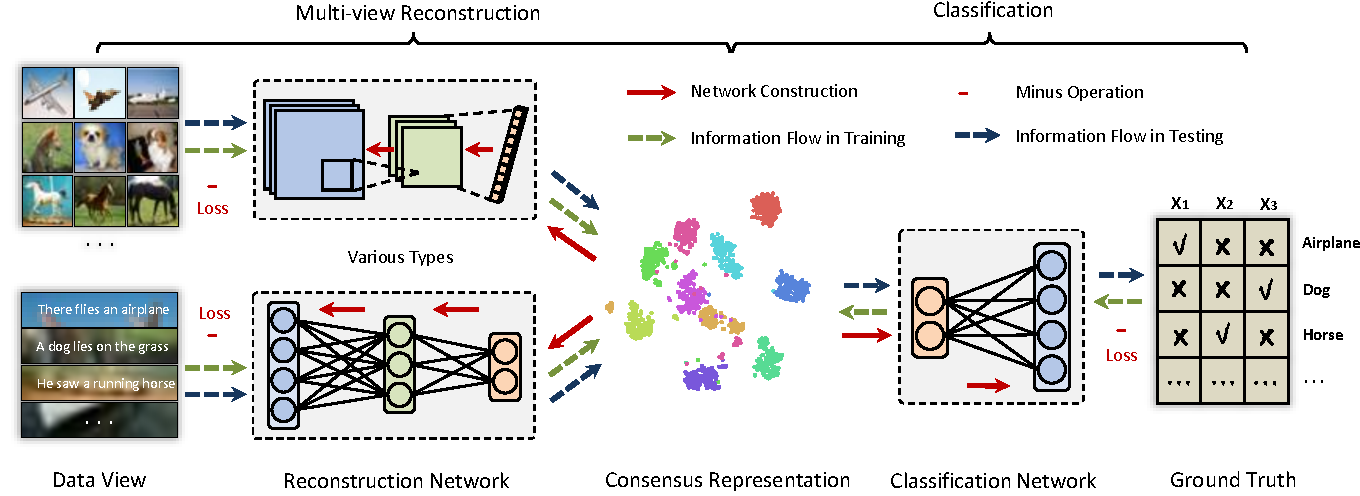
\includegraphics[width=\textwidth]{./fig/overview_gmnet.pdf}
\caption{Overview of the proposed General Multi-view Neural Network. }
\label{fig:overview_gmnet}
\end{figure}

\end{frame}


\begin{frame} \frametitle{General Multi-view Neural Network}

Formulation:

\begin{equation}
\begin{split}
  \min_{\mathbf{h}, \boldsymbol{\Theta}_c, \boldsymbol{\Theta}_r}\; \ell_c(\mathbf{y}, \mathbf{h}; \boldsymbol{\Theta}_c) + \lambda \sum_{v=1}^V \ell_r(\mathbf{X}_v, \mathbf{h}; \boldsymbol{\Theta}_r)
\end{split}
\end{equation}

in which 
\begin{equation}
\begin{split}
  & \ell_c(\mathbf{y}, \mathbf{h}; \boldsymbol{\Theta}_c) = \Delta (\mathbf{y}, g(\mathbf{h}; \boldsymbol{\Theta}_c)) \\
  & \ell_r(\mathbf{X}_v, \mathbf{h}; \boldsymbol{\Theta}_r) = \sum_{v=1}^V \|f_v(\mathbf{h}; \boldsymbol{\Theta}_r^{(v)}) - \mathbf{X}_v\|^2 \\
\end{split}
\end{equation}


\end{frame}


\section{Thanks}

\begin{frame}
    
    \centering
    \Huge Thanks !
    
\end{frame}





\end{document}